\chapter[Background]{Background}
\section{GraalVM Compiler Optimizations}

In GraalVM, the compilation process is divided into two main phases. The first phase, involving the Graal IR, handles most of the high-level optimizations. This phase is further organized into three tiers: high-tier for high-level optimizations, mid-tier for memory-focused enhancements, and low-tier for low-level IR (LIR) conversion \cite{Graal2021}. This project will primarily concentrate on high-tier optimizations within the GraalVM, beginning with the canonicalization phase. Canonicalization, an essential early phase in the optimization process, focuses on transforming code into a standardized format and eliminating redundancies. This transformation simplifies and facilitates the application of subsequent optimizations. Examples of canonicalization include:

\begin{description}
    \item \textbf{Constant Folding:} Replace constant expressions with their computed values, such as simplifying \newline
    \(3 + 4\) to \(7\).
    \item \textbf{Simplify Redundant Multiplication:} Eliminate unnecessary multiplication operations, such as converting \(x * 0\) to 0, and \(x * 1\) to \(x\).
    \item \textbf{Simplifying Conditional Statements:} Reduce complexity in conditional logic by removing redundant or always false branches. For example, an if statement with a condition that can never be true, such as \texttt{if (false)}, can be simplified by removing the entire branch.
    \item \textbf{Global Value Numbering:} Eliminate redundant computations by assigning unique identifiers to equivalent expressions \cite{Cliff1995}. For instance, if the expression \(a + b\) appears multiple times in the code, global value numbering ensures that it is computed only once and reused, thereby reducing unnecessary recalculations.
\end{description}

\section{Graal Intermediate Representation (IR)}

The Graal IR \cite{Duboscq2013} models a program's structure and operations using a directed graph that illustrates both data and control flow between nodes. Each node in this graph is designed to produce a single value and follows the Static Single Assignment (SSA) \cite{Ron1991} form. Data flow is represented by input edges pointing upward to the operand nodes, control flow is depicted by successor edges pointing downwards to the successor nodes. This IR framework provides a robust and efficient structure for code analysis and transformation, where optimization processes involve modifying the graph to enhance overall performance. A critical aspect of this project involves converting the Graal IR into Prolog facts to enable the optimizer to query these facts for potential optimizations. Therefore, it is essential to thoroughly understand the IR's structure and components to translate and use it within the Prolog-based optimization framework effectively.

\autoref{figure:graphir} illustrates a simple IR graph, with control flow edges highlighted in red. The graph begins at the Start node, which connects to the Return node via a successor edge. Upon reaching the Return node, the graph traverses upward through data flow edges to compute the returned expression’s value. This traversal demonstrates how control and data flows interact to process and complete the function's execution.

\begin{figure}[h]
    \centering
    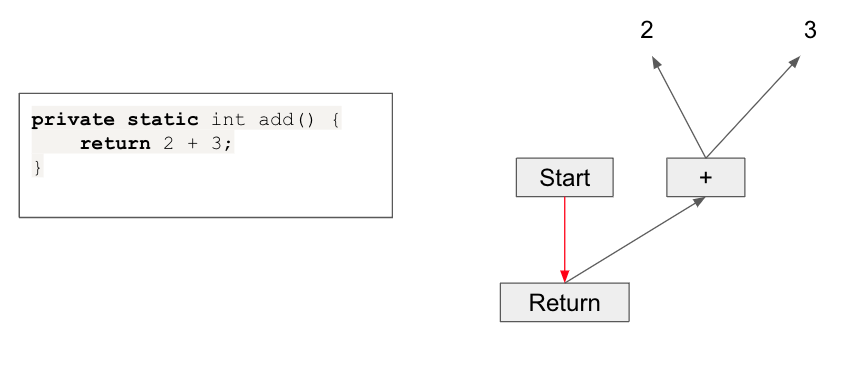
\includegraphics[width=0.9\textwidth]{Packages/graphir.png}
    \caption{Simple IR Graph}
    \label{figure:graphir}
\end{figure}

\section{Ahead-of-time (AOT) Compilation}
In the Java Virtual Machine (JVM), byte code compilation can occur either at build time or runtime. Ahead-of-time (AOT) compilation involves translating the byte code into machine code before execution, resulting in a fully compiled binary that is immediately executable \cite{Wade2017}. In contrast, Just-In-Time (JIT) Compilation defers the translation until runtime if at all, dynamically converting Java bytecodes into machine code within the JVM and optimizing frequently executed code paths to enhance performance \cite{Wade2017}. AOT compilation generally requires longer build times but offers rapid startup and predictable performance, making it suitable for applications where quick initialization is critical. JIT compilation, while benefiting from shorter build times, incurs longer startup periods but allows for more complex optimizations based on runtime profiling data.

AOT compilation is advantageous for this project as it performs all compilation and optimizations during the build phase, thereby minimizing runtime overhead. JIT compilation enables techniques such as speculative optimizations \cite{Duboscq2013Inproceedings}, which make assumptions about a program’s behavior to apply performance-enhancing transformations based on runtime profiling. Although these optimizations can significantly improve performance by optimizing frequently executed code paths, incorrect assumptions may necessitate deoptimizations, which revert the code to a less optimized but more reliable version~\cite{Duboscq2013Inproceedings}. This can complicate the program's IR by adding additional nodes and edges to accommodate these transformations \cite{Duboscq2013Inproceedings}. In this project, the emphasis will be on AOT compilation, where speculative optimizations are excluded \cite{Wimmer2019}, resulting in a simpler IR without the need for deoptimization. 

\section{Prolog Programming Language}

In traditional imperative languages, a program consists of a sequence of instructions.
This approach emphasizes a step-by-step procedure where each instruction modifies the state of the machine to solve a given problem. 
In contrast, logic programming languages, such as Prolog, operate on a fundamentally different paradigm. 
Instead of prescribing a sequence of operations, logic programming focuses on defining a knowledge base composed of facts and rules \cite{Bramer2013}. After that, users can query the knowledge base to search for objects and relations. 

In Prolog, facts represent objects and their relationships, while rules imply the relationship between objects given it satisfies all the conditions. Once the knowledge base is established, users can formulate queries to extract information or solve problems by leveraging the logical relationships defined in the base using the depth-first search algorithm \cite{Chowdhary2020}. There may be several ways to achieve a given goal. The system initially selects the first available option. If Prolog fails to resolve a specific subgoal, it will backtrack to explore these previously noted alternatives. This mechanism, referred to as backtracking \cite{Chowdhary2020}, enables Prolog to systematically search for different solutions by revisiting and trying alternative paths.

\begin{figure}[h]
    \centering
    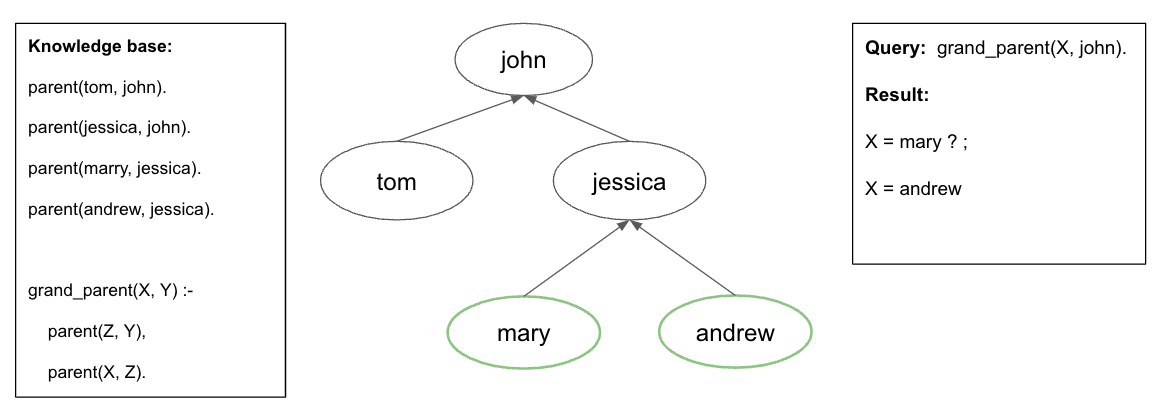
\includegraphics[width=1\textwidth]{Packages/Prolog.png}
    \caption{Example of Prolog specification}
    \label{figure:prolog}
\end{figure}

\autoref{figure:prolog} illustrates a Prolog program. The first three clauses are facts: john is a parent of tom and jessica, and jessica is a parent of both mary and andrew. The final clause is a rule defining the conditions for a grandparent relationship. When a query is made to determine the nodes for which john is a grandparent, Prolog performs a search from the first to the last clause, showcasing its backtracking behavior. Initially, Prolog identifies that john is a parent of tom, but since tom is not a parent of anyone, the search backtracks. It then considers the next option: jessica. Prolog then finds that jessica is a parent of mary. After exploring this path, Prolog backtracks again and continues to check the next possibility: jessica is also a parent of andrew, thereby completing the query.

\newpage
